\documentclass[conference]{IEEEtran}
\usepackage{graphicx}
\usepackage{amsmath}
\usepackage{amssymb}
\usepackage{url}
\usepackage{booktabs}
\usepackage{cite}

\begin{document}

\title{SkinSync: Profile-Aware Compatibility Scoring from Messy Cosmetic Ingredient Lists}

\author{\IEEEauthorblockN{Amaka Okoro}
\IEEEauthorblockA{COMP365 Individual Project}}

\maketitle

\begin{abstract}
Reading a cosmetic ingredient list is harder than it looks. The same chemical shows up under different names, and public catalogs have typos. I wanted to know if a short skin profile plus the INCI list is enough to say whether a product is a reasonable match, or if a single global ``bad ingredient'' list works just as well. SkinSync parses messy INCI strings, matches them to a small safety lexicon, and scores a product for a profile. I compared three methods on the same 54 pairs that I labeled myself: a keyword blacklist, a lexicon detector that ignores the person, and a profile-aware scorer. On a 19 pair holdout that I labeled after I froze the scoring weights, the profile-aware scorer got 0.947 accuracy. The other two got 0.684 and 0.632. I did not train a neural model. The labels are mine, the test set is small, and one holdout error shows that treating every EU listed allergen as fragrance is too blunt.
\end{abstract}

\begin{IEEEkeywords}
Ingredient Matching, Personalization, Cosmetic INCI, Fuzzy String Matching, Compatibility Scoring
\end{IEEEkeywords}

\section{Introduction}
I started this project because I kept seeing people treat ingredient lists like a simple yes or no. They look at the back of a bottle and try to decide if a moisturizer is ``safe for me.'' That is harder than it sounds. Aqua and Water are the same thing. Parfum, fragrance, and perfume get used for the same idea. Open Beauty Facts also has OCR style typos, like PERFUME or ISOPROPYL MYRSTATE. A blacklist is easy to write, but it treats everyone the same. Retinol is a problem if your barrier is already irritated. It is a goal if you are mainly worried about aging.

My research question is: given only an INCI string and a short skin profile, can a scorer that uses the profile tell compatible products from incompatible ones better than methods that ignore the person?

The AI task is binary classification of product and profile pairs. There is also a matching step that turns a free text INCI list into lexicon entries. I did not train a classifier from scratch. I did not fine tune a pretrained model. The string matching library is RapidFuzz~\cite{bachmann2025rapidfuzz}. I wrote the scoring rules and the labels.

What I built is SkinSync. It has an INCI parser, a keyword baseline, a lexicon detector that ignores the profile, and a 0 to 100 scorer that does use the profile. I typed 17 control products, cleaned 180 Open Beauty Facts records so I could test the parser, and labeled 54 pairs for four fake profiles. My contributions are the parser (it keeps 1,2-diol names and slash synonyms), the three way comparison on the same labels, and a holdout set that I wrote after I froze the penalty weights. Open Beauty Facts, RapidFuzz, scikit-learn~\cite{pedregosa2011sklearn}, and the EU allergen list~\cite{eu1223} are not my work.

\section{Related Work}
Lee et al. train a deep network on ordered cosmetic ingredients and add facial skin analysis for product recommendation~\cite{lee2024jcd}. That paper is peer reviewed in the \emph{Journal of Cosmetic Dermatology}. They are trying to guess how well a product will work, using a big catalog and a face image. I am not doing that. I do not use images and I did not train a network. My question is smaller: is this INCI list a reasonable match for this person.

Kalici\'{n}ska et al. predict whether one cosmetic ingredient is a sensitizer from chemical descriptors. Their best Naive Bayes model got 86\% accuracy~\cite{kalicinska2023ijms}. That paper is also peer reviewed (\emph{International Journal of Molecular Sciences}). They look at one chemical, not a full INCI list next to a user profile. I used published allergen lists instead of molecular descriptors. I cite this because it is a different approach. It shows a learned model can work at the chemical level. I did not try that.

Kyaw, Uttama, and Panwong treat ingredient lists as bags of terms and recommend products with TF-IDF plus cosine or Jaccard similarity~\cite{kyaw2024incit}. The conference paper is peer reviewed (IEEE InCIT 2024, Chonburi, Thailand). I also read the author posted master's thesis that reports the same skincare experiment~\cite{kyaw2024thesis}. Cosine similarity got 66.40\% average accuracy against specialist selections. Jaccard got 61.52\%. Both got 80\% on serum and sunscreen. That is a different setup from mine. They treat ingredient overlap as the signal. If two formulas look similar, they recommend the second one even if it has fragrance and the user cannot use fragrance. I score a named restriction list instead of finding nearest neighbor products.

Liu, Suresh, and Banitalebi-Dehkordi extract skin type and concern attributes from ingredient text for e-commerce recommendations~\cite{liu2024beauty}. That work was at the RecSys 2024 SURE workshop and is also on arXiv (2409.13628). I am treating it as a workshop paper / preprint, not a journal article. They compare a keyword pipeline to a learned attribute model on an expert annotated catalog. The learned model beat keywords. I kept the keyword idea as my baseline. I added an explicit user profile, which they do not score as compatible or not.

Most of these papers assume clean ingredients, recommend similar products, or predict general product attributes. I did not find much that tests messy, misspelled INCI strings against a personal restriction list. That is the gap I tried to fill, with a small rule based system. I only cite papers I opened and checked.

\section{Methodology}
\subsection{Data}
Public product records come from the Open Beauty Facts search API.\footnote{\url{https://world.openbeautyfacts.org/cgi/search.pl}} I dropped rows with fewer than five parsed ingredients or leftover packaging text. That left 180 products (mean 24.4 tokens). I also typed 11 products in an earlier checkpoint and 6 more for holdout testing. Those include CeraVe, Vanicream, The Ordinary, Paula's Choice, COSRX, La Roche-Posay, Aveeno, Olay, and a few generic formulas. I copied INCI text from labels or brand sites. There are no real users and no personal data. I did not need IRB approval. The four people in Table~\ref{tab:profiles} are made up.

I wrote those profiles. I labeled 35 development pairs while I was still changing the scorer. I labeled 19 holdout pairs after I froze the penalty table. A label of 1 means I would treat the product as a reasonable match for that profile. These are my labels, not clinical outcomes.

\begin{table}[t]
\caption{Synthetic Profiles Used for Every Labeled Pair}
\label{tab:profiles}
\centering
\scriptsize
\begin{tabular}{@{}llp{4.6cm}@{}}
\toprule
ID & Skin type & Restrictions / goal \\
\midrule
Maya & dry, sensitive & fragrance, alcohol; avoid leave-on retinol/BHA \\
Jordan & oily, acne-prone & comedogenic oils; can use BHA \\
Priya & combination & tree nut and soy allergy \\
Alex & normal & aging; retinol is desired \\
\bottomrule
\end{tabular}
\end{table}

\subsection{Cleaning and Matching}
The parser splits on commas, but it does not split inside parentheses or inside names like 1,2-Hexanediol. Aqua/Water and Parfum/Fragrance are stored as aliases. I strip percents and notes like ``(sunscreen).'' I left the typos in the messy control product on purpose.

Tokens get matched to a lexicon I tagged from EU Annex III fragrance allergens~\cite{eu1223} and common 0 to 5 comedogenic charts. Exact alias match is first. If that fails, RapidFuzz \texttt{token\_sort\_ratio} runs with cutoff 94. I tried 90 first. That matched sorbic acid to ascorbic acid, so I raised the cutoff and added a length check.

\subsection{Three Methods}
The rubric asks for at least three models under the same evaluation. I compare three decision methods, not three trained models. None of M1, M2, or M3 is fit from data. I picked them so I could change one thing at a time. M1 is the first thing I would have written. M2 uses the same lexicon as M3 but still ignores the person. If M3 is better than M2, that has to come from the profile. M3 is the system I actually built. All three get the same raw INCI string. M3 also gets the profile. I did not train any of them. I did not use a pretrained language model.

\textbf{M1. Keyword baseline.} A hardcoded substring list (fragrance, retinol, SLS, coconut oil, and similar terms). Any hit scores 0. Otherwise 100. No profile. I used this because a lot of label checkers work this way, and Liu et al. also start from keywords~\cite{liu2024beauty}.

\textbf{M2. Profile-blind lexicon.} Same parser and fuzzy matcher as M3. Any risk tagged ingredient (fragrance, irritant, retinoid, comedogenic oil, and similar tags) makes the product incompatible. No profile. I added this so a better matcher would not get counted as personalization.

\textbf{M3. Profile-aware scorer.} Start at 100. Subtract penalties only when a matched ingredient matters for that profile (listed sensitivity, acne vs comedogenic oils, reactive skin vs leave-on retinol or BHA). Add a little for ceramides, niacinamide, and humectants. I call a pair compatible if the score is at least 60 and there is no ``avoid'' flag. I set the weights by hand on the 35 pair development set, then I froze them.

\subsection{Splits, Leakage, and Evaluation}
Nothing is trained, so there is no random train/test split. To keep myself from tuning on the test labels, I wrote the 19 holdout labels after I froze M3. The development labels are still a problem. I wrote those while I was writing the rules. Leave one product out on the 35 pair set is perfect for M3. I am not reporting that as evidence. Removing a product does not re-estimate any parameter.

I report label accuracy and precision, recall, and F1 on the unsafe class (gold label 0). The holdout set has 16 compatible pairs and 3 incompatible pairs. Unsafe F1 on 3 positives is fragile, so I also report raw counts. Missing an incompatible product is worse than being a little conservative. scikit-learn computes the F1 numbers~\cite{pedregosa2011sklearn}. All three methods are scored on the same 35 + 19 pairs.

\subsection{Implemented Parts, Tools, and Hardware}
I implemented the INCI parser, the lexicon tags, M1, M2, M3, the 54 labels, the evaluation script, and a small FastAPI demo. I did not implement a trained classifier, a second annotator, concentration parsing, or leave-on vs rinse-off detection.

I ran everything on CPU, Linux, Python 3.12.3, RapidFuzz 3.14.6, scikit-learn 1.9.1, and pandas 3.0.6. No GPU. Pinned versions are in \texttt{requirements.txt}. To repeat the numbers: \texttt{PYTHONPATH=. python3 -m skinsync.evaluate\_final}. The RapidFuzz cutoff is 94. A pair is compatible if the score is at least 60 and there is no avoid flag. Claude helped me debug the parser and the eval scripts. I wrote the labels, the lexicon tags, and the penalty table. The penalty table in commit \texttt{checkpoint1-frozen-weights} is the same table I used on the holdout.

The main method limits are the author labels, a drugstore heavy catalog, and a lexicon that cannot see concentration or whether a product is rinse off.

\section{Results}
Table~\ref{tab:main} and Figure~\ref{fig:bars} show the three methods on the same pairs. On the 35 pair development set, M1 and M2 both get 0.829 accuracy (29/35). M3 matches all 35 labels. That last number is not that impressive. I wrote those labels while I was looking at the same products.

The holdout set is the fairer comparison. It has 16 compatible pairs and 3 incompatible pairs (Maya and the AHA peel, Maya and Olay Regenerist, Jordan and Aveeno). Table~\ref{tab:holdout} has the unsafe class numbers. M1 is right on 13 of 19 pairs (accuracy 0.684, unsafe precision 0.286, recall 0.667, F1 0.400). M2 is right on 12 of 19 (0.632; precision 0.300, recall 1.000, F1 0.462). M3 is right on 18 of 19 (0.947; precision 0.750, recall 1.000, F1 0.857). Across all 54 pairs the accuracies are 0.778, 0.759, and 0.981. M2 is one pair worse than M1 on the holdout. The extra misses are Maya and Priya on Aveeno. M2 flags isopropyl palmitate and benzyl alcohol for everyone. M1 does not catch those tokens, so it calls both pairs compatible. Alex and retinol is a development example in Table~\ref{tab:examples}, not a holdout pair. On the holdout, M1 and M2 both reject Jordan and the AHA peel, which I labeled compatible, and M3 accepts it. That is also why I do not think Kyaw et al. are answering the same question~\cite{kyaw2024incit}. Similar formulas are not the same thing as ``safe for this person.''

\begin{table}[t]
\caption{Three Methods on the Same Product and Profile Labels}
\label{tab:main}
\centering
\scriptsize
\begin{tabular}{@{}l ccc ccc@{}}
\toprule
 & \multicolumn{3}{c}{Accuracy} & \multicolumn{3}{c}{Unsafe F1} \\
\cmidrule(lr){2-4}\cmidrule(lr){5-7}
Method & Dev & Hold. & All & Dev & Hold. & All \\
\midrule
M1 Keyword & 0.829 & 0.684 & 0.778 & 0.824 & 0.400 & 0.727 \\
M2 Blind lexicon & 0.829 & 0.632 & 0.759 & 0.824 & 0.462 & 0.723 \\
M3 Profile-aware & 1.000 & 0.947 & 0.981 & 1.000 & 0.857 & 0.971 \\
\bottomrule
\end{tabular}\\[2pt]
{\scriptsize Dev $n{=}35$. Holdout $n{=}19$. All $n{=}54$.}
\end{table}

\begin{table}[t]
\caption{Holdout Unsafe Class Precision, Recall, and F1 (3 Unsafe Pairs)}
\label{tab:holdout}
\centering
\scriptsize
\begin{tabular}{@{}lccc@{}}
\toprule
Method & Precision & Recall & F1 \\
\midrule
M1 Keyword & 0.286 & 0.667 & 0.400 \\
M2 Blind lexicon & 0.300 & 1.000 & 0.462 \\
M3 Profile-aware & 0.750 & 1.000 & 0.857 \\
\bottomrule
\end{tabular}\\[2pt]
{\scriptsize Holdout $n{=}19$ (16 compatible, 3 incompatible). Unsafe class is gold label 0.}
\end{table}

\begin{figure}[t]
\centering
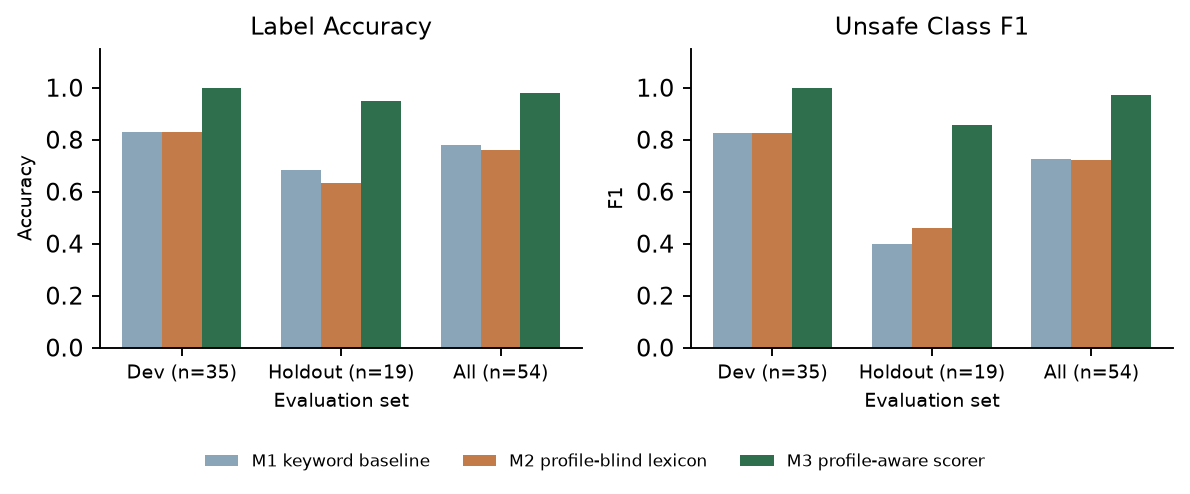
\includegraphics[width=\columnwidth]{final_three_models.png}
\caption{Label Accuracy (Left) and Unsafe Class F1 (Right) for M1, M2, and M3 on Dev ($n{=}35$), Holdout ($n{=}19$), and All 54 Pairs. Gray is M1, Orange is M2, Green is M3}
\label{fig:bars}
\end{figure}

Figure~\ref{fig:bars} is the same accuracy and unsafe F1 numbers as Table~\ref{tab:main}. Left bars are development. Middle bars are holdout. Right bars are all 54 pairs. M3 is highest in every group. The biggest gap is holdout F1, where M1 drops to 0.400.

Table~\ref{tab:examples} has example outputs. Maya and CeraVe Moisturizing Cream is the easy yes. All three methods call it compatible. M3 scores 100 with no flags. Maya and the messy OCR lotion is the easy no. It has perfume and several EU allergens. Alex and a 0.5\% retinol serum is the case that shows why the profile matters. M1 and M2 both reject it because retinol is on a global risk list. M3 scores 100 and calls it compatible, which matches the label I wrote for someone who wants retinol.

\begin{table}[t]
\caption{Example Outputs for the Same INCI Strings}
\label{tab:examples}
\centering
\scriptsize
\begin{tabular}{@{}llp{1.15cm}p{1.15cm}p{1.35cm}@{}}
\toprule
Profile & Product & M1 & M2 & M3 (score) \\
\midrule
Maya & CeraVe cream & yes & yes & yes (100) \\
Maya & Messy lotion & no & no & no (0) \\
Alex & Retinol serum & no & no & yes (100) \\
Maya & Aveeno lotion & yes & no & no (65) \\
Maya & Retinol serum & no & no & no$^*$ (86) \\
\bottomrule
\end{tabular}\\[2pt]
{\scriptsize $^*$Binary flag is ``no''; printed verdict still says good match.}
\end{table}

The parser ran on all 180 Open Beauty Facts products (mean 24.4 tokens, mean 6.0 lexicon hits). I did not label those 180 rows, so I am not reporting accuracy on them.

Table~\ref{tab:fail} lists the two weak cases I actually saw. The holdout error is Maya and Aveeno. The score and flag mismatch is Maya and retinol. That second one is already in the development set.

I cannot say M3 is accurate in general. The 1.00 on the development set uses labels I wrote for the same products I used to set the weights. The holdout 18/19 result is more useful, and it is still small.

\section{Discussion}
The holdout numbers support the research question a little. Using the profile improved accuracy by 0.263 over the keyword baseline and by 0.315 over the profile-blind lexicon. That gain is not from finding more risk ingredients. M2 already finds those and then rejects too much. The gain is from not counting retinol, BHA, or a fragrance free comedogenic oil against someone who has no reason to avoid it.

The holdout failure is Maya and Aveeno Daily Moisturizing Lotion (Table~\ref{tab:fail}). I labeled that pair compatible. M3 scored 65, printed ``use with caution,'' and called it incompatible because benzyl alcohol is tagged as a fragrance allergen. In that formula benzyl alcohol is a preservative. I have not tested a fix. One idea is to tag preservative uses separately from perfume. Another is to require a second fragrance hit before rejecting the product. I did not put either change into the numbers above.

\begin{table}[t]
\caption{Observed Weak Cases, Not Hypothetical Ones}
\label{tab:fail}
\centering
\scriptsize
\begin{tabular}{@{}p{2.05cm}p{3.15cm}p{2.15cm}@{}}
\toprule
Pair & What happened & Status \\
\midrule
Maya $\times$ Aveeno & Gold 1; M3 says no (score 65) because benzyl alcohol is tagged as a fragrance allergen & holdout error; fix not tested \\
Maya $\times$ retinol & Gold 0; flag is avoid, but score is 86 and the verdict still says good match & rule bug; fix not tested \\
\bottomrule
\end{tabular}
\end{table}

The second problem is already in the development set. For Maya and the 0.5\% retinol serum, the binary flag is right (incompatible, avoid retinol). The numeric score is still 86 and the printed verdict is ``good match'' because humectant bonuses raise the number. The same thing happens for Maya and a BHA exfoliant (78), Jordan and an almond cream (79), and Priya and the messy soy lotion (78). If I ranked Maya's products by score, retinol would sit near the top even though I already labeled it unsafe. I have not tested a corrected verdict rule. The fix I would try first is to block ``good match'' when an avoid flag is present.

Every compatibility label is mine. There is no second annotator and no clinical outcome. Open Beauty Facts lists are incomplete, so I cannot treat the 180 public products as a labeled test set. The typed catalog is mostly drugstore and The Ordinary.

A clear ingredient check could help people read labels. A wrong ``safe'' score on an allergen would be bad. SkinSync is not a medical device.

Next I want to do two specific things. First, change the verdict rule so an avoid flag cannot print ``good match,'' and retag preservative benzyl alcohol. Second, have another person label at least 50 new pairs and score a labeled slice of the Open Beauty Facts dump. I have not run either step yet.

\section{Conclusion}
SkinSync scores cosmetic INCI lists against a skin profile. On 19 holdout pairs that I labeled after I froze the weights, the profile-aware scorer beat a keyword blacklist and a lexicon that ignores the person. The labels are mine, the Aveeno error is real, and the 0 to 100 score can disagree with the yes or no flag. Those limits should stay attached to the result.

\begin{thebibliography}{00}
\bibitem{lee2024jcd}
Jinhee Lee, Huisu Yoon, Semin Kim, Chanhyeok Lee, Jongha Lee, and Sangwook Yoo, ``Deep Learning-Based Skin Care Product Recommendation: A Focus on Cosmetic Ingredient Analysis and Facial Skin Conditions,'' \emph{Journal of Cosmetic Dermatology}, vol.~23, no.~6, pp.~2066--2077, 2024.

\bibitem{kalicinska2023ijms}
Jadwiga Kalici\'{n}ska, Barbara Wi\'{s}niowska, Sebastian Polak, and Radoslaw Spiewak, ``Artificial Intelligence That Predicts Sensitizing Potential of Cosmetic Ingredients with Accuracy Comparable to Animal and In Vitro Tests,'' \emph{International Journal of Molecular Sciences}, vol.~24, no.~7, art.~6801, 2023.

\bibitem{kyaw2024incit}
Theint Zar Lwin Kyaw, Surapong Uttama, and Patcharaporn Panwong, ``Leveraging Ingredient Profiles in Content-Based Skincare Product Recommendation,'' in \emph{Proc. 8th Int. Conf. Information Technology (InCIT)}, Chonburi, Thailand, 2024, p.~319.

\bibitem{kyaw2024thesis}
Theint Zar Lwin Kyaw, ``Leveraging Cosmetic Ingredient Profiles and Skin-Related Features for Cosmetic Products Recommendation,'' M.S. thesis, School of Applied Digital Technology, Mae Fah Luang Univ., Chiang Rai, Thailand, 2024. Author posted full text used to verify the InCIT experiment.

\bibitem{liu2024beauty}
Celine Liu, Rahul Suresh, and Amin Banitalebi-Dehkordi, ``Beauty Beyond Words: Explainable Beauty Product Recommendations Using Ingredient-Based Product Attributes,'' in \emph{Proc. SURE Workshop at ACM RecSys}, Bari, Italy, 2024, arXiv:2409.13628. Workshop paper / preprint.

\bibitem{bachmann2025rapidfuzz}
Max Bachmann, ``rapidfuzz/RapidFuzz,'' Zenodo, 2025, doi:10.5281/zenodo.15133267.

\bibitem{pedregosa2011sklearn}
Fabian Pedregosa, Ga\"{e}l Varoquaux, Alexandre Gramfort, Vincent Michel, Bertrand Thirion, Olivier Grisel, Mathieu Blondel, Peter Prettenhofer, Ron Weiss, Vincent Dubourg, Jake Vanderplas, Alexandre Passos, David Cournapeau, Matthieu Brucher, Matthieu Perrot, and \'{E}douard Duchesnay, ``Scikit-learn: Machine Learning in Python,'' \emph{Journal of Machine Learning Research}, vol.~12, pp.~2825--2830, 2011.

\bibitem{eu1223}
European Parliament and Council, ``Regulation (EC) No 1223/2009 on Cosmetic Products,'' \emph{Official Journal of the European Union}, L~342, pp.~59--209, Dec.~22, 2009.
\end{thebibliography}

\clearpage
\onecolumn
\section*{Supplemental Materials (Course Submission Only)}
This page is not part of the IEEE SoutheastCon 2027 manuscript. COMP365 requires the demo and reproducibility links after the paper.

\subsection*{Venue}
IEEE SoutheastCon 2027, regular paper track, at most 6 pages. Manuscript deadline December 31, 2026, 11:59 p.m. US Eastern. Conference April 15 to 18, 2027, Daytona Beach, FL. The review copy for ExOrdo is double-blind. The camera ready copy keeps the author name. Call for papers: \url{https://ieeesoutheastcon.org/call-for-papers/}. Submission instructions: \url{https://ieeesoutheastcon.org/paper-submission-instructions/}.

\subsection*{Overleaf}
The manuscript is written in the IEEE conference template (\texttt{IEEEtran}, conference option). The Overleaf project contains \texttt{skinsync\_southeastcon.tex}, \texttt{IEEEtran.cls}, and \texttt{final\_three\_models.png}. Dr. Pope and the teaching assistants have edit access on that project.

\subsection*{Recorded Demo and Paper Review}
The live demo and paper review is a 6 to 10 minute recording in the author's own voice. The speaking outline used for that recording is \texttt{demo/SCRIPT.md}. No text to speech.

\textbf{Demo video:} not published yet. Record from \texttt{demo/SCRIPT.md}, upload unlisted, then put the tested URL on this line before Canvas.

\subsection*{Reproducible Materials}
The public materials needed to rebuild the system and repeat Table~\ref{tab:main} are the \texttt{skinsync/} package, \texttt{skinsync/catalog.py} (54 labels), \texttt{skinsync/lexicon.py}, \texttt{data/raw/open\_beauty\_facts\_products.json}, and \texttt{python3 -m skinsync.evaluate\_final}. Setup, pinned versions, RapidFuzz cutoff 94, score threshold 60, and hardware are in the repository README. The commit tagged \texttt{checkpoint1-frozen-weights} is the scorer before the holdout labels were written.

\textbf{Repository:} not published to public GitHub yet. This environment cannot create that remote. After the public repo exists, put the clone URL on this line.

Claude was used on the code (parser and evaluation scripts). I wrote the labels and the scoring rules.

\end{document}
